% -*-cap2.tex-*-
% Este fichero es parte de la plantilla LaTeX para
% la realización de Proyectos Final de Carrera, protejido
% bajo los términos de la licencia GFDL.
% Para más información, la licencia completa viene incluida en el
% fichero fdl-1.3.tex

% Copyright (C) 2009 Pablo Recio Quijano 

\section{Organización temporal}

En este apartado podemos añadir un diagrama de Gannt, con la
planificación temporal que se realizó del proyecto. Para ello podemos
usar algún programa libre como por ejemplo \programa{Planner}:

\figura{gannt.png}{scale=0.6}{Diagrama de Gannt. Desarrollo del
  proyecto}{gannt}{H}

Observad el código, notareis algo distinto con respecto a las imágenes
del capítulo anterior. En este caso utilizo un comando personalizado
en \comando{comandos.sty}, donde simplifico la creación de una
figura, como en la figura~\ref{gannt}. % Podemos poner o no la ~

\section{Análisis del sistema}

Si el proyecto se refiere a un sistema software, normalmente
procederemos a un análisis y a un diseño del sistema usando notación
UML, para organizar correctamente dicho sistema.\\

\LaTeX{} no trae soporte nativo para hacer este tipo de diagramas, y
aunque se pueden utilizar paquetes que lo hagan. Sin embargo lo más
cómodo es que utilizemos herramientas CASE para ayudarnos a dicha
tarea, como pueden ser \programa{Dia} o \programa{Umbrello}, como
podemos ver en la figura \ref{uml}.

\figura{uml.png}{scale=1}{UML de ejemplo con Umbrello}{uml}{H}

Ya que no es el objetivo de este documento trabajar con dichas
herramientas, aprovecharé este apartado para mostrar algunas
cosas más de las que podemos dotar a nuestro documento \LaTeX{}.\\

Sabemos que tenemos un fichero \texttt{bibliografia.bib}, para que la
herramienta Bib\TeX{}  nos genere las referencias bibliográficas. Sin
embargo a priori no se mostrarán hasta que nos las referenciemos.\\

Teniendo en cuenta que todo esto lo tomamos desde la ``biblia'' de
\LaTeX, podemos hacer una referencia a ella \cite{mitt04}. También hay
que saber que una guia de referencia online muy buena es la página en
\texttt{wikibooks} de \LaTeX{} \cite{website:latex-wikibooks}. 

% TO-DO: Multirow, Multicolumn y Supertabular.

\section{Base de Datos}

Supongamos que en este apartado, queremos incluir un \negrita{diagrama
Entidad-Relación Extendido}, que modele la base de datos que vamos a
utilizar en nuestro proyecto. Una posible herramienta para dibujarla
es \programa{Dia}, una herramienta pra gráficos vectoriales bastante
completa. Una vez hemos hecho el diagrama, podemos importarlo a una
imagen en multitud de formatos, o también podemos a código
\programa{.tex}.\\

¿Qué utilidad tiene esto? Pues basicamente lo podremos modificar para
refinarlo un poco, añadirle fórmulas matemáticas si quisieramos, o
diversas cosas. Además de comprimir bastante en espacio respecto a una
imagen. El diagrama \ref{ERe}, está realizado con Dia importándolo a
\LaTeX{}:

\begin{figure}[H]
  \label{ERe}
  \begin{center}
    % -*-ERe.tex-*-
% Este fichero es parte de la plantilla LaTeX para
% la realización de Proyectos Final de Carrera, protejido
% bajo los términos de la licencia GFDL.
% Para más información, la licencia completa viene incluida en el
% fichero fdl-1.3.tex

% Copyright (C) 2009 Pablo Recio Quijano, Noelia Sales Montes

% necesita \usepackage{tikz}
\ifx\du\undefined
  \newlength{\du}
\fi
\setlength{\du}{15\unitlength}
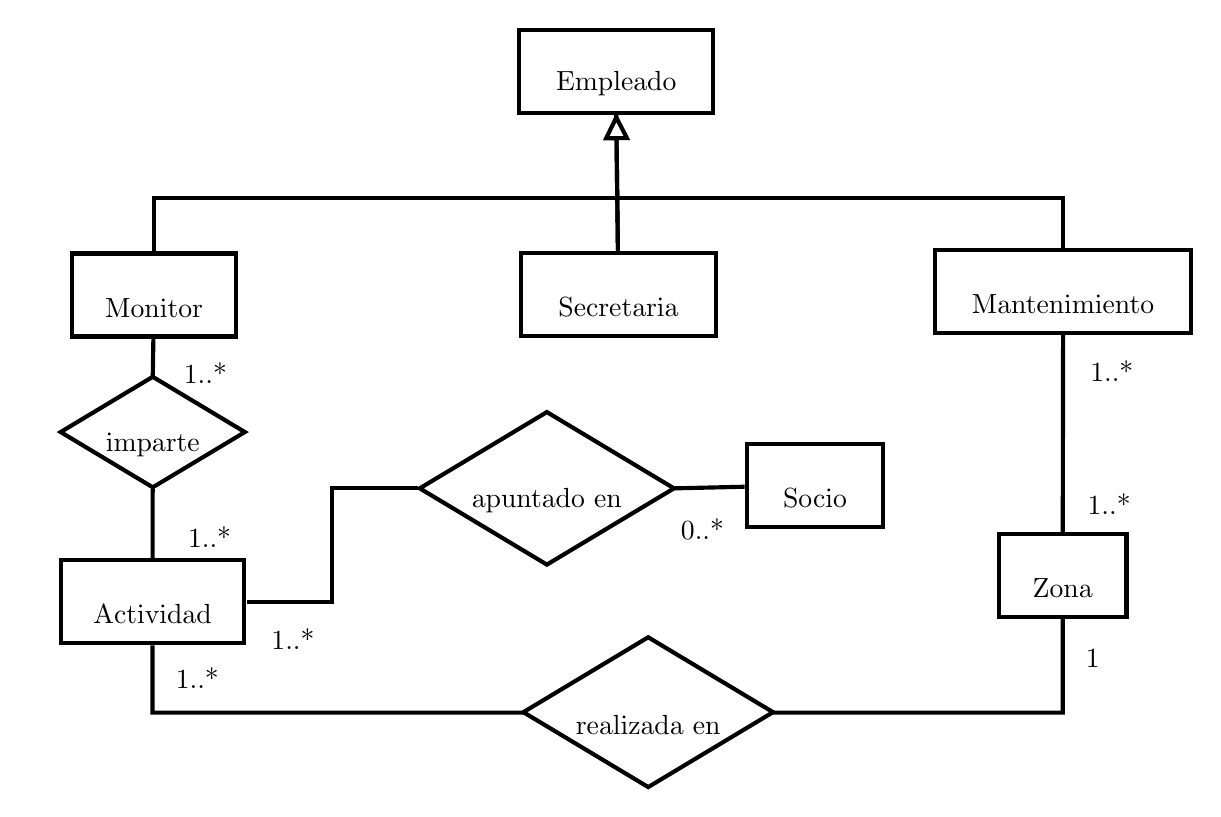
\begin{tikzpicture}
\pgftransformxscale{1.000000}
\pgftransformyscale{-1.000000}
\definecolor{dialinecolor}{rgb}{0.000000, 0.000000, 0.000000}
\pgfsetstrokecolor{dialinecolor}
\definecolor{dialinecolor}{rgb}{1.000000, 1.000000, 1.000000}
\pgfsetfillcolor{dialinecolor}
\definecolor{dialinecolor}{rgb}{1.000000, 1.000000, 1.000000}
\pgfsetfillcolor{dialinecolor}
\fill (20.800000\du,-5.900000\du)--(20.800000\du,-3.900000\du)--(25.475000\du,-3.900000\du)--(25.475000\du,-5.900000\du)--cycle;
\pgfsetlinewidth{0.100000\du}
\pgfsetdash{}{0pt}
\pgfsetmiterjoin
\definecolor{dialinecolor}{rgb}{0.000000, 0.000000, 0.000000}
\pgfsetstrokecolor{dialinecolor}
\draw (20.800000\du,-5.900000\du)--(20.800000\du,-3.900000\du)--(25.475000\du,-3.900000\du)--(25.475000\du,-5.900000\du)--cycle;
% setfont left to latex
\definecolor{dialinecolor}{rgb}{0.000000, 0.000000, 0.000000}
\pgfsetstrokecolor{dialinecolor}
\node at (23.137500\du,-4.597500\du){Empleado};
\definecolor{dialinecolor}{rgb}{1.000000, 1.000000, 1.000000}
\pgfsetfillcolor{dialinecolor}
\fill (20.840000\du,-0.530000\du)--(20.840000\du,1.470000\du)--(25.542500\du,1.470000\du)--(25.542500\du,-0.530000\du)--cycle;
\pgfsetlinewidth{0.100000\du}
\pgfsetdash{}{0pt}
\pgfsetmiterjoin
\definecolor{dialinecolor}{rgb}{0.000000, 0.000000, 0.000000}
\pgfsetstrokecolor{dialinecolor}
\draw (20.840000\du,-0.530000\du)--(20.840000\du,1.470000\du)--(25.542500\du,1.470000\du)--(25.542500\du,-0.530000\du)--cycle;
% setfont left to latex
\definecolor{dialinecolor}{rgb}{0.000000, 0.000000, 0.000000}
\pgfsetstrokecolor{dialinecolor}
\node at (23.191250\du,0.772500\du){Secretaria};
\definecolor{dialinecolor}{rgb}{1.000000, 1.000000, 1.000000}
\pgfsetfillcolor{dialinecolor}
\fill (10.030000\du,-0.510000\du)--(10.030000\du,1.490000\du)--(13.980000\du,1.490000\du)--(13.980000\du,-0.510000\du)--cycle;
\pgfsetlinewidth{0.100000\du}
\pgfsetdash{}{0pt}
\pgfsetmiterjoin
\definecolor{dialinecolor}{rgb}{0.000000, 0.000000, 0.000000}
\pgfsetstrokecolor{dialinecolor}
\draw (10.030000\du,-0.510000\du)--(10.030000\du,1.490000\du)--(13.980000\du,1.490000\du)--(13.980000\du,-0.510000\du)--cycle;
% setfont left to latex
\definecolor{dialinecolor}{rgb}{0.000000, 0.000000, 0.000000}
\pgfsetstrokecolor{dialinecolor}
\node at (12.005000\du,0.792500\du){Monitor};
\definecolor{dialinecolor}{rgb}{1.000000, 1.000000, 1.000000}
\pgfsetfillcolor{dialinecolor}
\fill (30.822600\du,-0.595000\du)--(30.822600\du,1.405000\du)--(36.982600\du,1.405000\du)--(36.982600\du,-0.595000\du)--cycle;
\pgfsetlinewidth{0.100000\du}
\pgfsetdash{}{0pt}
\pgfsetmiterjoin
\definecolor{dialinecolor}{rgb}{0.000000, 0.000000, 0.000000}
\pgfsetstrokecolor{dialinecolor}
\draw (30.822600\du,-0.595000\du)--(30.822600\du,1.405000\du)--(36.982600\du,1.405000\du)--(36.982600\du,-0.595000\du)--cycle;
% setfont left to latex
\definecolor{dialinecolor}{rgb}{0.000000, 0.000000, 0.000000}
\pgfsetstrokecolor{dialinecolor}
\node at (33.902600\du,0.707500\du){Mantenimiento};
\definecolor{dialinecolor}{rgb}{1.000000, 1.000000, 1.000000}
\pgfsetfillcolor{dialinecolor}
\fill (32.354000\du,6.245200\du)--(32.354000\du,8.245200\du)--(35.431500\du,8.245200\du)--(35.431500\du,6.245200\du)--cycle;
\pgfsetlinewidth{0.100000\du}
\pgfsetdash{}{0pt}
\pgfsetmiterjoin
\definecolor{dialinecolor}{rgb}{0.000000, 0.000000, 0.000000}
\pgfsetstrokecolor{dialinecolor}
\draw (32.354000\du,6.245200\du)--(32.354000\du,8.245200\du)--(35.431500\du,8.245200\du)--(35.431500\du,6.245200\du)--cycle;
% setfont left to latex
\definecolor{dialinecolor}{rgb}{0.000000, 0.000000, 0.000000}
\pgfsetstrokecolor{dialinecolor}
\node at (33.892750\du,7.547700\du){Zona};
\definecolor{dialinecolor}{rgb}{1.000000, 1.000000, 1.000000}
\pgfsetfillcolor{dialinecolor}
\fill (26.282700\du,4.070200\du)--(26.282700\du,6.070200\du)--(29.570200\du,6.070200\du)--(29.570200\du,4.070200\du)--cycle;
\pgfsetlinewidth{0.100000\du}
\pgfsetdash{}{0pt}
\pgfsetmiterjoin
\definecolor{dialinecolor}{rgb}{0.000000, 0.000000, 0.000000}
\pgfsetstrokecolor{dialinecolor}
\draw (26.282700\du,4.070200\du)--(26.282700\du,6.070200\du)--(29.570200\du,6.070200\du)--(29.570200\du,4.070200\du)--cycle;
% setfont left to latex
\definecolor{dialinecolor}{rgb}{0.000000, 0.000000, 0.000000}
\pgfsetstrokecolor{dialinecolor}
\node at (27.926450\du,5.372700\du){Socio};
\pgfsetlinewidth{0.100000\du}
\pgfsetdash{}{0pt}
\pgfsetdash{}{0pt}
\pgfsetbuttcap
{
\definecolor{dialinecolor}{rgb}{0.000000, 0.000000, 0.000000}
\pgfsetfillcolor{dialinecolor}
% was here!!!
\definecolor{dialinecolor}{rgb}{0.000000, 0.000000, 0.000000}
\pgfsetstrokecolor{dialinecolor}
\draw (23.178300\du,-0.580358\du)--(23.137500\du,-3.900000\du);
}
\definecolor{dialinecolor}{rgb}{0.000000, 0.000000, 0.000000}
\pgfsetstrokecolor{dialinecolor}
\draw (23.178300\du,-0.580358\du)--(23.145019\du,-3.288243\du);
\pgfsetmiterjoin
\definecolor{dialinecolor}{rgb}{1.000000, 1.000000, 1.000000}
\pgfsetfillcolor{dialinecolor}
\fill (23.395000\du,-3.291315\du)--(23.138874\du,-3.788205\du)--(22.895038\du,-3.285170\du)--cycle;
\pgfsetlinewidth{0.100000\du}
\pgfsetdash{}{0pt}
\pgfsetmiterjoin
\definecolor{dialinecolor}{rgb}{0.000000, 0.000000, 0.000000}
\pgfsetstrokecolor{dialinecolor}
\draw (23.395000\du,-3.291315\du)--(23.138874\du,-3.788205\du)--(22.895038\du,-3.285170\du)--cycle;
\pgfsetlinewidth{0.100000\du}
\pgfsetdash{}{0pt}
\pgfsetdash{}{0pt}
\pgfsetmiterjoin
\pgfsetbuttcap
{
\definecolor{dialinecolor}{rgb}{0.000000, 0.000000, 0.000000}
\pgfsetfillcolor{dialinecolor}
% was here!!!
{\pgfsetcornersarced{\pgfpoint{0.000000\du}{0.000000\du}}\definecolor{dialinecolor}{rgb}{0.000000, 0.000000, 0.000000}
\pgfsetstrokecolor{dialinecolor}
\draw (33.902600\du,-0.595000\du)--(33.902600\du,-1.839800\du)--(12.005000\du,-1.839800\du)--(12.005000\du,-0.559434\du);
}}
\definecolor{dialinecolor}{rgb}{1.000000, 1.000000, 1.000000}
\pgfsetfillcolor{dialinecolor}
\fill (9.754000\du,3.791450\du)--(11.972750\du,2.460200\du)--(14.191500\du,3.791450\du)--(11.972750\du,5.122700\du)--cycle;
\pgfsetlinewidth{0.100000\du}
\pgfsetdash{}{0pt}
\pgfsetmiterjoin
\definecolor{dialinecolor}{rgb}{0.000000, 0.000000, 0.000000}
\pgfsetstrokecolor{dialinecolor}
\draw (9.754000\du,3.791450\du)--(11.972750\du,2.460200\du)--(14.191500\du,3.791450\du)--(11.972750\du,5.122700\du)--cycle;
% setfont left to latex
\definecolor{dialinecolor}{rgb}{0.000000, 0.000000, 0.000000}
\pgfsetstrokecolor{dialinecolor}
\node[anchor=east] at (9.454000\du,3.491450\du){};
\definecolor{dialinecolor}{rgb}{0.000000, 0.000000, 0.000000}
\pgfsetstrokecolor{dialinecolor}
\node[anchor=west] at (14.491500\du,3.491450\du){};
\definecolor{dialinecolor}{rgb}{0.000000, 0.000000, 0.000000}
\pgfsetstrokecolor{dialinecolor}
\node at (11.972750\du,4.093950\du){imparte};
\pgfsetlinewidth{0.100000\du}
\pgfsetdash{}{0pt}
\pgfsetdash{}{0pt}
\pgfsetbuttcap
{
\definecolor{dialinecolor}{rgb}{0.000000, 0.000000, 0.000000}
\pgfsetfillcolor{dialinecolor}
% was here!!!
\definecolor{dialinecolor}{rgb}{0.000000, 0.000000, 0.000000}
\pgfsetstrokecolor{dialinecolor}
\draw (11.987836\du,1.538593\du)--(11.972750\du,2.460200\du);
}
\pgfsetlinewidth{0.100000\du}
\pgfsetdash{}{0pt}
\pgfsetdash{}{0pt}
\pgfsetbuttcap
{
\definecolor{dialinecolor}{rgb}{0.000000, 0.000000, 0.000000}
\pgfsetfillcolor{dialinecolor}
% was here!!!
\definecolor{dialinecolor}{rgb}{0.000000, 0.000000, 0.000000}
\pgfsetstrokecolor{dialinecolor}
\draw (11.970796\du,5.169007\du)--(11.968437\du,6.832059\du);
}
\definecolor{dialinecolor}{rgb}{1.000000, 1.000000, 1.000000}
\pgfsetfillcolor{dialinecolor}
\fill (18.404000\du,5.147700\du)--(21.466500\du,3.310200\du)--(24.529000\du,5.147700\du)--(21.466500\du,6.985200\du)--cycle;
\pgfsetlinewidth{0.100000\du}
\pgfsetdash{}{0pt}
\pgfsetmiterjoin
\definecolor{dialinecolor}{rgb}{0.000000, 0.000000, 0.000000}
\pgfsetstrokecolor{dialinecolor}
\draw (18.404000\du,5.147700\du)--(21.466500\du,3.310200\du)--(24.529000\du,5.147700\du)--(21.466500\du,6.985200\du)--cycle;
% setfont left to latex
\definecolor{dialinecolor}{rgb}{0.000000, 0.000000, 0.000000}
\pgfsetstrokecolor{dialinecolor}
\node[anchor=east] at (18.104000\du,4.847700\du){};
\definecolor{dialinecolor}{rgb}{0.000000, 0.000000, 0.000000}
\pgfsetstrokecolor{dialinecolor}
\node[anchor=west] at (24.829000\du,4.847700\du){};
\definecolor{dialinecolor}{rgb}{0.000000, 0.000000, 0.000000}
\pgfsetstrokecolor{dialinecolor}
\node at (21.466500\du,5.450200\du){apuntado en};
\pgfsetlinewidth{0.100000\du}
\pgfsetdash{}{0pt}
\pgfsetdash{}{0pt}
\pgfsetbuttcap
{
\definecolor{dialinecolor}{rgb}{0.000000, 0.000000, 0.000000}
\pgfsetfillcolor{dialinecolor}
% was here!!!
\definecolor{dialinecolor}{rgb}{0.000000, 0.000000, 0.000000}
\pgfsetstrokecolor{dialinecolor}
\draw (24.529000\du,5.147700\du)--(26.232300\du,5.108850\du);
}
\pgfsetlinewidth{0.100000\du}
\pgfsetdash{}{0pt}
\pgfsetdash{}{0pt}
\pgfsetmiterjoin
\pgfsetbuttcap
{
\definecolor{dialinecolor}{rgb}{0.000000, 0.000000, 0.000000}
\pgfsetfillcolor{dialinecolor}
% was here!!!
{\pgfsetcornersarced{\pgfpoint{0.000000\du}{0.000000\du}}\definecolor{dialinecolor}{rgb}{0.000000, 0.000000, 0.000000}
\pgfsetstrokecolor{dialinecolor}
\draw (11.966970\du,8.929609\du)--(11.967000\du,10.550000\du)--(33.892750\du,10.550000\du)--(33.892750\du,8.245200\du);
}}
\definecolor{dialinecolor}{rgb}{1.000000, 1.000000, 1.000000}
\pgfsetfillcolor{dialinecolor}
\fill (20.900700\du,10.539700\du)--(23.908200\du,8.735200\du)--(26.915700\du,10.539700\du)--(23.908200\du,12.344200\du)--cycle;
\pgfsetlinewidth{0.100000\du}
\pgfsetdash{}{0pt}
\pgfsetmiterjoin
\definecolor{dialinecolor}{rgb}{0.000000, 0.000000, 0.000000}
\pgfsetstrokecolor{dialinecolor}
\draw (20.900700\du,10.539700\du)--(23.908200\du,8.735200\du)--(26.915700\du,10.539700\du)--(23.908200\du,12.344200\du)--cycle;
% setfont left to latex
\definecolor{dialinecolor}{rgb}{0.000000, 0.000000, 0.000000}
\pgfsetstrokecolor{dialinecolor}
\node[anchor=east] at (20.600700\du,10.239700\du){};
\definecolor{dialinecolor}{rgb}{0.000000, 0.000000, 0.000000}
\pgfsetstrokecolor{dialinecolor}
\node[anchor=west] at (27.215700\du,10.239700\du){};
\definecolor{dialinecolor}{rgb}{0.000000, 0.000000, 0.000000}
\pgfsetstrokecolor{dialinecolor}
\node at (23.908200\du,10.842200\du){realizada en};
\pgfsetlinewidth{0.100000\du}
\pgfsetdash{}{0pt}
\pgfsetdash{}{0pt}
\pgfsetbuttcap
{
\definecolor{dialinecolor}{rgb}{0.000000, 0.000000, 0.000000}
\pgfsetfillcolor{dialinecolor}
% was here!!!
\definecolor{dialinecolor}{rgb}{0.000000, 0.000000, 0.000000}
\pgfsetstrokecolor{dialinecolor}
\draw (33.902600\du,1.405000\du)--(33.894521\du,6.195076\du);
}
\definecolor{dialinecolor}{rgb}{1.000000, 1.000000, 1.000000}
\pgfsetfillcolor{dialinecolor}
\fill (9.753200\du,6.880200\du)--(9.753200\du,8.880200\du)--(14.180700\du,8.880200\du)--(14.180700\du,6.880200\du)--cycle;
\pgfsetlinewidth{0.100000\du}
\pgfsetdash{}{0pt}
\pgfsetmiterjoin
\definecolor{dialinecolor}{rgb}{0.000000, 0.000000, 0.000000}
\pgfsetstrokecolor{dialinecolor}
\draw (9.753200\du,6.880200\du)--(9.753200\du,8.880200\du)--(14.180700\du,8.880200\du)--(14.180700\du,6.880200\du)--cycle;
% setfont left to latex
\definecolor{dialinecolor}{rgb}{0.000000, 0.000000, 0.000000}
\pgfsetstrokecolor{dialinecolor}
\node at (11.966950\du,8.182700\du){Actividad};
\pgfsetlinewidth{0.100000\du}
\pgfsetdash{}{0pt}
\pgfsetdash{}{0pt}
\pgfsetmiterjoin
\pgfsetbuttcap
{
\definecolor{dialinecolor}{rgb}{0.000000, 0.000000, 0.000000}
\pgfsetfillcolor{dialinecolor}
% was here!!!
{\pgfsetcornersarced{\pgfpoint{0.000000\du}{0.000000\du}}\definecolor{dialinecolor}{rgb}{0.000000, 0.000000, 0.000000}
\pgfsetstrokecolor{dialinecolor}
\draw (14.231000\du,7.880200\du)--(16.294100\du,7.880200\du)--(16.294100\du,5.147700\du)--(18.357300\du,5.147700\du);
}}
% setfont left to latex
\definecolor{dialinecolor}{rgb}{0.000000, 0.000000, 0.000000}
\pgfsetstrokecolor{dialinecolor}
\node[anchor=west] at (12.450000\du,2.368750\du){1..*};
% setfont left to latex
\definecolor{dialinecolor}{rgb}{0.000000, 0.000000, 0.000000}
\pgfsetstrokecolor{dialinecolor}
\node[anchor=west] at (34.285000\du,2.331250\du){1..*};
% setfont left to latex
\definecolor{dialinecolor}{rgb}{0.000000, 0.000000, 0.000000}
\pgfsetstrokecolor{dialinecolor}
\node[anchor=west] at (34.220000\du,5.516250\du){1..*};
% setfont left to latex
\definecolor{dialinecolor}{rgb}{0.000000, 0.000000, 0.000000}
\pgfsetstrokecolor{dialinecolor}
\node[anchor=west] at (12.255000\du,9.713750\du){1..*};
% setfont left to latex
\definecolor{dialinecolor}{rgb}{0.000000, 0.000000, 0.000000}
\pgfsetstrokecolor{dialinecolor}
\node[anchor=west] at (12.550100\du,6.331250\du){1..*};
% setfont left to latex
\definecolor{dialinecolor}{rgb}{0.000000, 0.000000, 0.000000}
\pgfsetstrokecolor{dialinecolor}
\node[anchor=west] at (24.425000\du,6.133750\du){0..*};
% setfont left to latex
\definecolor{dialinecolor}{rgb}{0.000000, 0.000000, 0.000000}
\pgfsetstrokecolor{dialinecolor}
\node[anchor=west] at (14.560000\du,8.768750\du){1..*};
% setfont left to latex
\definecolor{dialinecolor}{rgb}{0.000000, 0.000000, 0.000000}
\pgfsetstrokecolor{dialinecolor}
\node[anchor=west] at (34.180000\du,9.238750\du){1};
\end{tikzpicture}

    % Comentar si no está el paquete tkiz instalado, y descomentar la
    % linea siguiente. Comentar además la inclusión del paquete en
    % estilos/estiloBase.sty
    %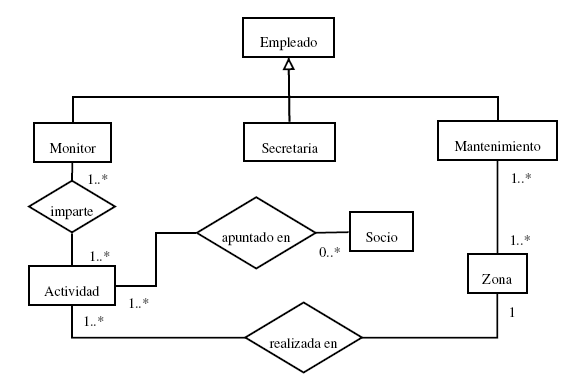
\includegraphics[scale=0.8]{ERe.png}
  \end{center}
  \caption{Diagrama ERe de ejemplo}
\end{figure}


\section{Código fuente}

En \LaTeX tenemos varias maneras de colocar nuestro código fuente, pero
vamos a mostrar dos básicas.

\subsection{Entorno \texttt{Verbatim}}

Este entorno, nos permite incluir dentro de él \negrita{cualquier}
código, y nos respetará espacios, saltos de lineas, tabuladores... es
decir, el compilador de \LaTeX no procesará ese entorno y lo dejará
tal cual está. Veamos un ejemplo con el clásico programa
\programa{Hola mundo} en \texttt{C++}:

\begin{verbatim}
/*Clásico programa en su versión C++*/

#include <iostream>

using namespace std;

int main()
{
  cout << "¡Hola, mundo!" << endl;
  return 0; //No hace falta, pero en fin
}
\end{verbatim}

Vemos, que queda un poco ``soso'': no remarca palabras del lenguaje,
le da igual lo que es comentario y lo que es texto, y claro, a la hora
de tener un código relativamente amplio, pues es incomodo verlo tan
plano. Hay alternativas como \texttt{fncyverbatim}, en la cual podemos
formatearlo algo, añadiendo números de lineas, remarcando palabras del
lenguaje y más opciones, pero quizás la siguiente opción sea más
completa:

\subsection{Entorno \texttt{listing}}

Si vemos en el fichero \comando{comandos.sty}, podemos ver varios
estilos definidos para este entorno. ¿En qué consiste? Pues realmente
este entorno, sabiendo de que lenguaje le estamos pasando el código
(admitiendo gran variedad como C, C++, Java, \TeX, SQL, ADA, Python y
muchísimos más), y ciertas opciones, podemos formatear el código.\\

Este entorno podemos llamarlo de dos formas distintas, la primera es
utilizando un entorno propiamente dicho, con sus
$\backslash$\texttt{begin} y $\backslash$\texttt{end} dentro del cual
copiamos el código, y otra usando el comando
$\backslash$\texttt{lstinputlisting}, pasándole de parámetro el propio
fichero. Veamos de las dos formas:

\begin{lstlisting}[style=C++]
/*Clasico programa en su version C++*/

#include <iostream>

using namespace std;

int main()
{
  cout << "Hola, mundo!" << endl;
  return 0; //No hace falta, pero en fin
}  
\end{lstlisting}

O de la segunda forma:

\lstinputlisting[style=C++]{hola_mundo.cpp}

Notar que uso el estilo \texttt{C++} porque ya lo tengo definido en el
fichero mencionado anteriormente, pero se pueden añadir varios más,
modificando los colores, si queremos o no número de lineas, o por
ejemplo comandos de consola:

\begin{lstlisting}[style=consola]
  g++ hola_mundo.cpp -o hola_mundo
\end{lstlisting}

Desde luego, es bastante más agradable para la vista, lo cual facilita
si lectura. Sin embargo, si usamos esta última opción probablemente
tengamos problemas con los caracteres españoles, acentos y demás,
debido a las diferencias de codificación entre ISO Latin-1 y UTF8. Hay
que tener cuidado en tenerlo todo en UTF8 para que el compilador
``entienda'' los caracteres.